\lstset{ %
language=[mips]Assembler,         % the language of the code
}
In the section \ref{sec:splitting} the code is divided in frames and after
that in basic blocks. It is also possible to create a graph from the whole code.
If this is done, it is possible to perform optimalisations on the graph. We 
implemented two optimalisations in the module \code{optimise\_tree}.
\subsubsection{Remove not used}
A program has only one entry point: the beginning of the instruction list. The 
first block should be the only block with no incoming edges. If there are more
blocks with no incoming edges, then these can be removed since they will never 
be reached. The blocks with no edges are the blocks that are between a jump
and a label in the assembly code:
\begin{lstlisting}
    addu    $2,$3,4
    j       $L6
|   bne     $2,$0,$L5
|   mtc1    $2,$f0
|   lw      $31,52($sp)
|   lw      $fp,48($sp)
|   .loc    1 5
|   .ent    main        
$L6:
    div.d   $f0,$f0,$f2	
\end{lstlisting}
In this case, there are two lines that contain raw code. This code is used by
gcc and can therefore not be removed. So we keep \texttt{.loc} and \texttt{.end} 
and we remove \texttt{bne}, \texttt{mtc1} and the \texttt{lw} instructions. If
the raw types wouldn't be there, the jump would now be optimised in 
\ref{sec:global}.
\subsubsection{Flatten the graph}
For all blocks that have one incoming edge (now: "block two") and a block on the 
other side that has only one outgoing edge (now: "block one"), the blocks can 
be placed after eachother in the code. This can work out well when the only 
edge to a block is caused by a jump. This jump will become redundant if the 
blocks are repositioned. We implented this by appending all instructions from 
block two to the instructions from block one and by removing block two as a 
block object. 
\subsubsection{Result}
We made a code that generates a diagram from our graph when the verbosity level
is three. We generate a diagram image before and 
after optimalisation. The result is displayed for pi.s in a \ref{fig:before} 
and \ref{fig:after}.
\begin{figure}[H]
\centering
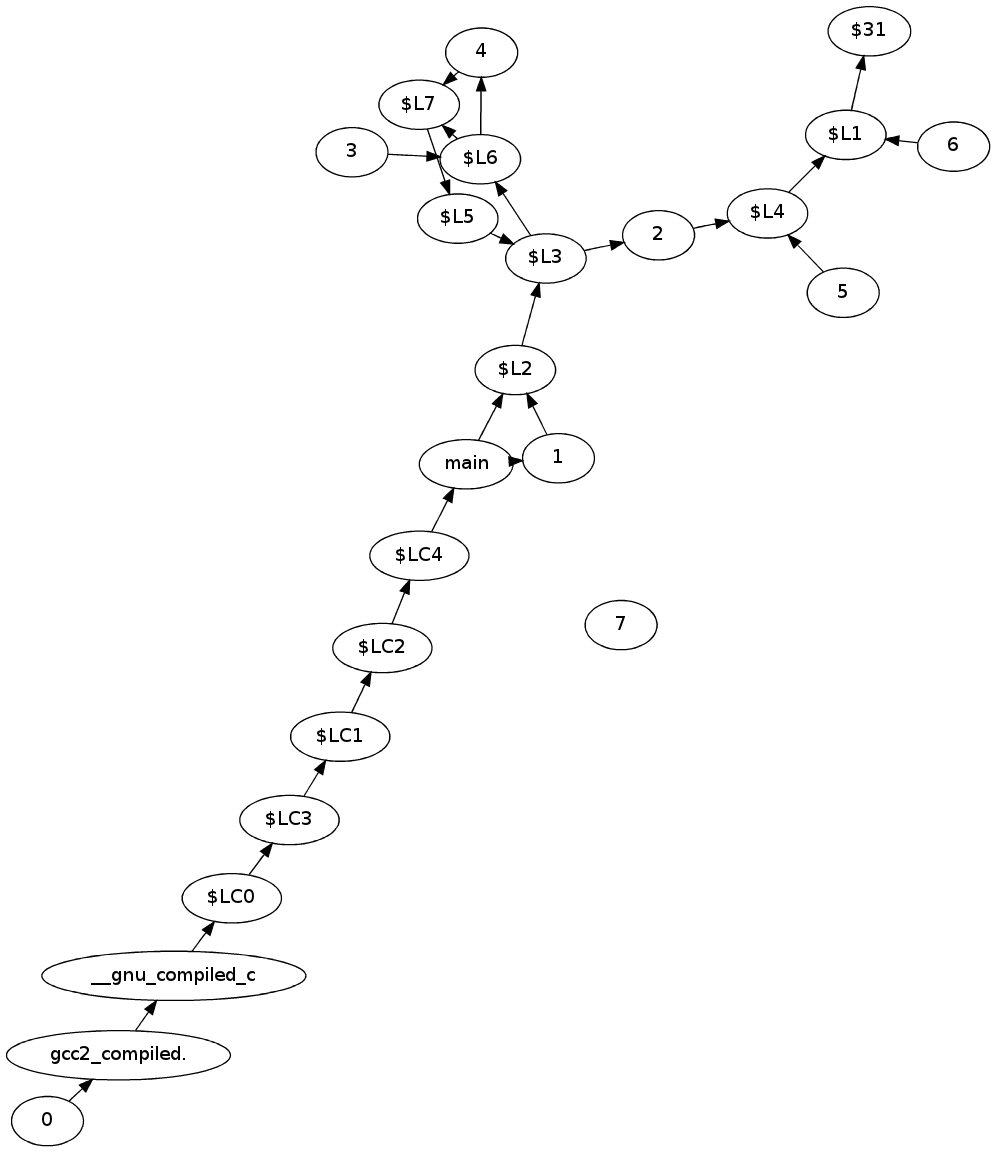
\includegraphics[scale=0.2]{images/before}
\caption{CFG for pi.s before optimalisation}
\label{fig:before}
\end{figure}
\begin{figure}[H]
\centering
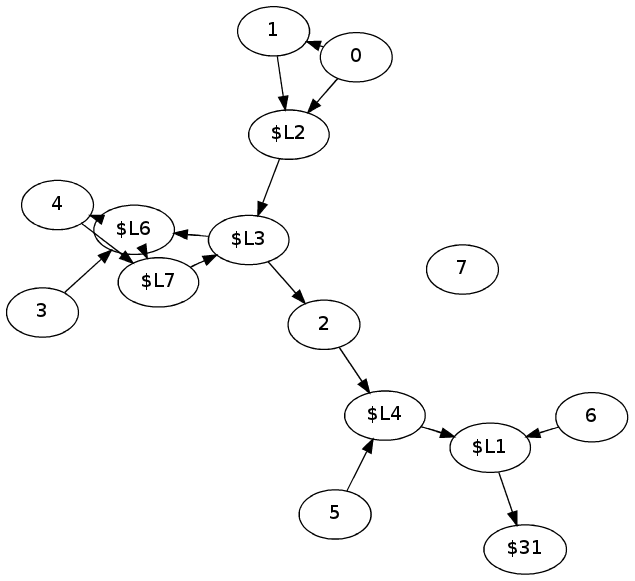
\includegraphics[scale=0.2]{images/after}
\caption{CFG for pi.s after optimalisation}
\label{fig:after}
\end{figure}
After the graph optimalisations we need to perform global jump optimalisations
to actually gain performance.

